\subsection{Bilanzierung}

\subsubsection{Kontext der Bilanzierung}

Bilanzierung ist ein Konzept welches in unterschiedlichen Einsatzbereichen verwendung findet. Diese Forschung befasst sich mit Bilanzräumen 
im Kontext der DIN EN ISO 50001:2018-12. Die Norm setzt den Schwerpunkt auf die fortlaufenden Verbesserung der energiebezogenen Leistung 
(\cite[Kapitel 0.2]{DIN50001.2018}). Aufgrund dessen sollte die Bilanzierung in diesem Forschungskontext aus einer Perspektive betrachtet werden welche 
energiebezogene Größen betrachtet.

Auch die Festlegung auf Organisationen des tertiären Wirtschaftssektors hat auswirkungen auf die betrachtungsweise der Bilanzierung. 
Denn in Organisation mit immateriellen Dienstleistungen spielt die Gebäudeenergie eine vorrangige Rolle zur Verbesserung der energiebezogenen 
Leistung (\cite[S. 3]{Fichera.2020}). 
Dies lässt sich Beispielhaft an der Abbildung \eqref{fig:Energieverbrauch_Wärme_DE} darstellen.

\begin{figure}[H]
    \centering
    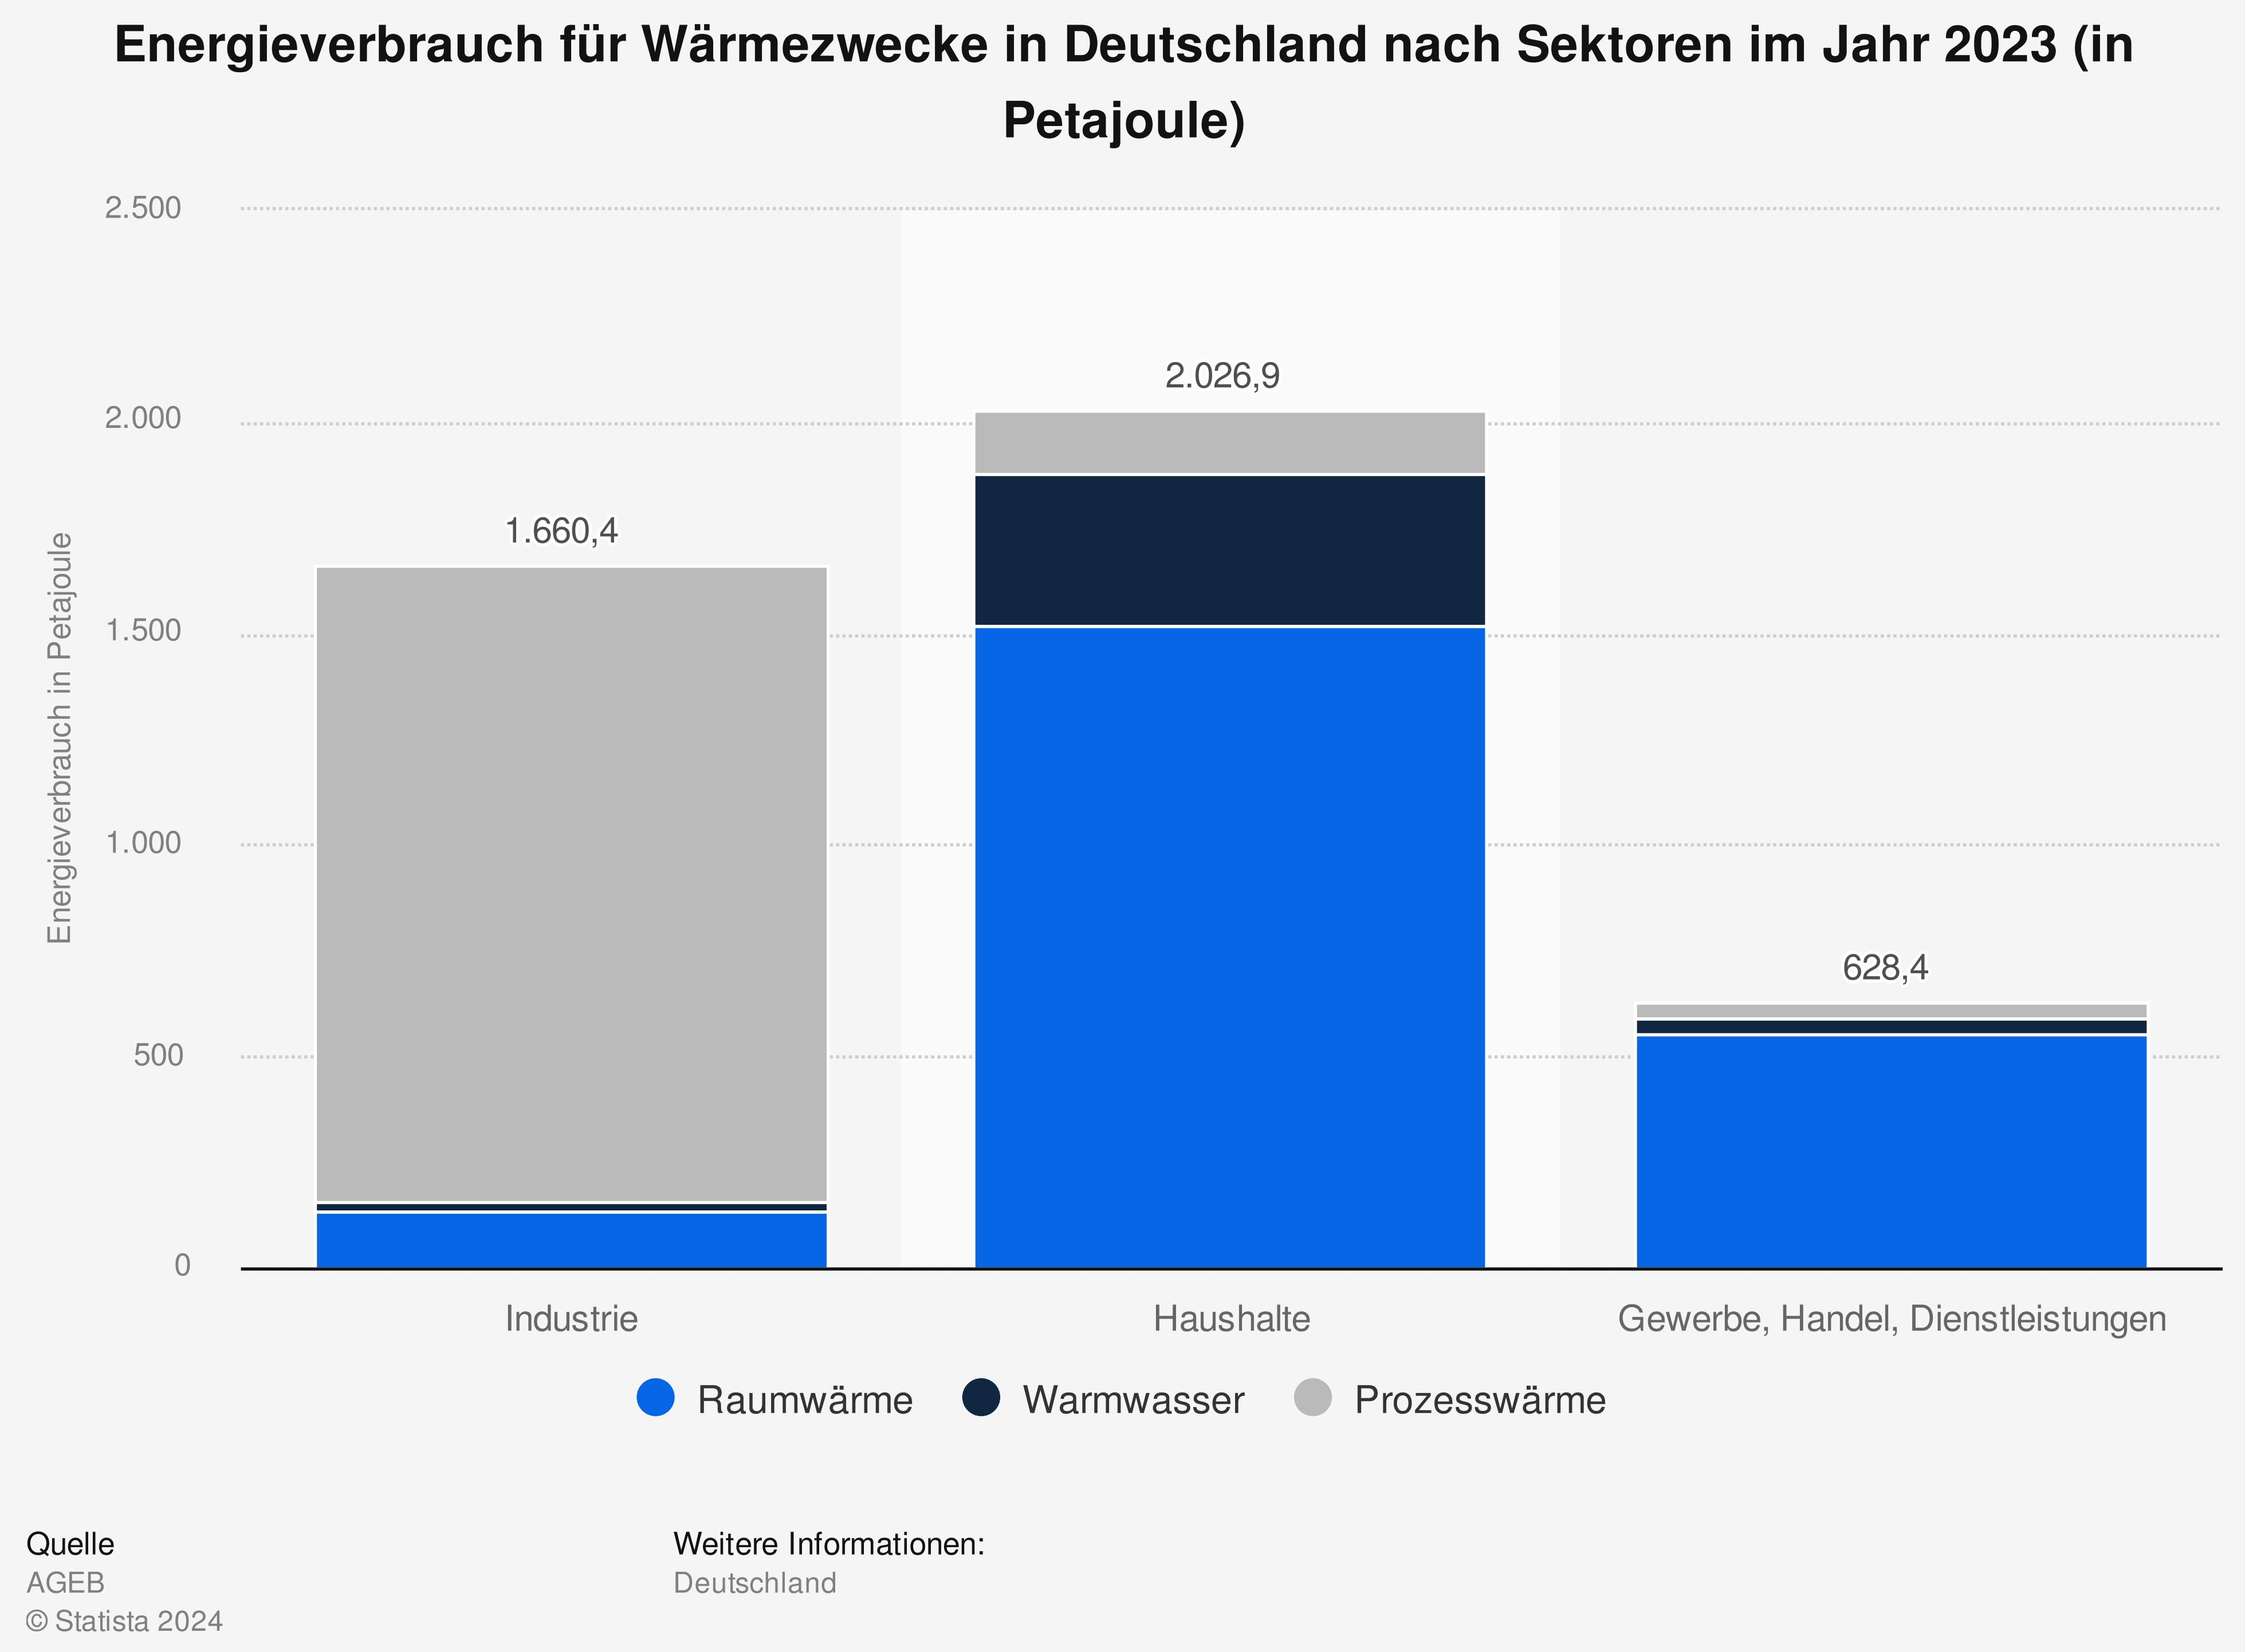
\includegraphics[width=0.68\textwidth]{../../Ressourcen/Bilder/Energieverbrauch_für_Wärmezweck_DE.jpg}
    \caption{Energieverbrauch für den Wärmezweck in Deutschland [\cite{AGEB.2024}]}
    \label{fig:Energieverbrauch_Wärme_DE}
\end{figure}

Die Abbildung \ref{fig:Energieverbrauch_Wärme_DE} zeigt den Energieverbrauch für Wärmezwecke in Deutschland im Jahr 2023, aufgeschlüsselt nach Sektoren. 
Während der industrielle Sektor einen hohen Anteil an prozessbezogener Wärme aufweist, spielt im Dienstleistungssektor die Raumwärme 
eine dominante Rolle.
Diese Statistik bekräftigt die Aussage von Fichera (2020, S. 3) dass bei der Verbesserung der energiebezogenen Leistung in Organisationen des tertiären 
Wirtschaftssektors energiebezogene Prozesse und Technologien im Gegensatz zur Gebäudeenergie eine untergeordnete Bedeutung haben. 

Im Rahmen der Bestimmung des Gesamtenergiebedarfs eines Gebäudes über den Lebenszyklus wird vor allem der Gebäudebetrieb betrachtet \cite[S. 133]{Musall.2015}.
Die sogenannte Graue Energie wird üblicherweise als kumulierter, nicht erneuerbarer Primärenergieaufwand beschrieben, der alle vor- und nachgelagerten 
Prozesse der verwendeten Baustoffe und Materialien sowie der technischen Anlagen umfasst \cite[S. 133]{Musall.2015}. Da sich die Norm auf die 
fortlaufende Verbesserung der energiebezogenen Leistung abzielt und die Graue Energie konstant ist wird diese im Rahmen dieser Arbeit nicht 
betrachtet. 
Stattdessen liegt der Fokus dieser Forschungsarbeit auf der Bilanzierung energetischer Größen im Rahmen von Organisation des tertiäten Wirtschaftssektors. 
Sie grenzt sich somit von der Bilanzierung von Rohstoffen und Materialien ab.

\subsubsection{Definition}
Im Rahmen des beschrieben Kontexts rückt die verfahrenstechnische Perspektive der Bilanzierung in den Fokus. 
So wird die Bilanzierung im Kontext der Verfahrenstechnik nach Rönsch (2015, S. 66) in drei Bilanzgleichungen unterteilt: 
die Massenbilanz, die Energiebilanz und die Impulsbilanz. 
Zur Beantwortung dieser Forschungsfrage hat insbesondere die Energiebilanz eine hohe Relevanz.

Die Energiebilanz beruht auf dem Energieerhaltungssatz (\cite[S. 66]{Rönsch.2015}), der das Prinzip der Erhaltung 
der Energie ausdrückt (\cite[S. 57]{Baehr.1966}). Der Energieerhaltungssatz bezieht sich auf alle Erscheinungsformen, in denen Energie auftritt, 
und besagt, dass es unmöglich ist, Energie zu erzeugen oder zu vernichten (\cite[S. 57]{Baehr.1966}). 
Für zu bilanzierende Systeme bedeutet dies, dass die Energie in einem abgeschlossenen, adiabaten System über die Zeit 
konstant ist (\cite[S. 66]{Rönsch.2015}). 
Adiabat bedeutet in diesem Kontext, dass das System keinen Wärme mit seiner Umgebung austauscht (\cite[S. 66]{Rönsch.2015}). 

Für Systeme, die in der Lage sind, Energie zu speichern, impliziert dies nach Rönsch (2015, S. 66f.), 
dass die darin gespeicherte Energie gleich der Differenz aus ein- und austretenden Energieströmen ist. 
Für offene, nicht-adiabate Systeme ohne Speicherfähigkeit gilt, dass die Differenz der ein- und austretenden Energieströme Null ist 
(\cite[S. 66f.]{Rönsch.2015}).
Das von Rönsch (2015, S. 66f.) beschriebene Verhalten eines Systems bezüglich der Energiespeicherung, lässt sich mathematisch 
vereinfacht mit der Gleichung \eqref{energiebilanzierungsgleichung_Rönsch} darstellen:

\begin{equation}
E_{\text{gespeichert}} = \sum E_{\text{eingang}} - \sum E_{\text{ausgang}}
\label{energiebilanzierungsgleichung_Rönsch}
\end{equation}

\begin{description}
    \item \(E_{\text{gespeichert}}\): Im System gespeicherte Energie.
    \item \(E_{\text{eingang}}\): Energie eines eintretenden Energiestroms.
    \item \(E_{\text{ausgang}}\): Energie eines austretenden Energiestroms.
    \item Für offene, nicht-adiabate Systeme ohne Energiespeicher gilt:
    \[
    E_{\text{gespeichert}} = 0
    \]
    \item In diesem Fall ist die zugeführte Energie gleich der abgegebenen Energie:
    \[
    \sum E_{\text{eingang}} = \sum E_{\text{ausgang}}
    \]
\end{description}

Diese Gleichung beschreibt einen allgemeinen Ansatz zur Energiebilanzierung der im System gespeicherten Energie. 
Im Rahmen der Bilanzierung komplexer Systeme kann jedoch eine detailliertere Bilanzierung einzelner Zustandsgrößen im System erforderlich sein.

Dieses Problem wird von der von Ahrendts (2014, Kapitel 1.5) aufgestellten Bilanzgleichung im Kontext der Thermodynamik addressiert. 
Die Gleichung basiert auf dem Fakt, dass sich für jede mengenartige Zustandsgröße, die über die Grenze eines Systems transportiert wird, eine 
Bilanz aufstellen lässt (\cite[Kapitel 1.5]{Ahrendts.2014}). 
Diese Bilanz umfasst ein- und austretende Ströme sowie im System enthaltene Energiequellen und -senken und ermittelt die 
Geschwindigkeit der Änderung des Bestands der zu bilanzierenden Zustandsgröße im System (\cite[Kapitel 1.5]{Ahrendts.2014}).

Die von Ahrendts (2014, Kapitel 1.5) aufgestellte Bilanzgleichung wird in den Formeln \eqref{BilanzierungsgleichungAhrendt} und 
\eqref{BilanzierungsgleichungAhrendtStrom} dargestellt.

\begin{equation}
    dX_{\text{j}}/d\tau = (\sum \dot{X}_{\text{j,e}} - \sum \dot{X}_{\text{j,a}}) + (\dot{X}_{\text{j,Quell}} - \dot{X}_{\text{j,Senk}})
    \label{BilanzierungsgleichungAhrendt}
\end{equation}

\begin{description}
    \item \(X_{\text{j}}\): Zustandsgröße.
    \item \(X_{\text{j,e}}\): Über die Systemgrenze zufließende Zustandsgröße.
    \item \(X_{\text{j,a}}\): Über die Systemgrenze abfließende Zustandsgröße.
    \item \(X_{\text{j,Quell}}\): Quellen der Zustandsgröße im System.
    \item \(X_{\text{j,Senk}}\): Senken der Zustandsgröße im System.
\end{description}

\begin{equation}
    \dot{X}_{\text{j}} = \lim_{\Delta\tau \to 0} \Delta X_{\text{j}}/ \Delta\tau
    \label{BilanzierungsgleichungAhrendtStrom}
\end{equation}

\begin{description}
    \item \(X_{\text{j}}\): Zustandsgröße.
    \item \(\Delta X_{\text{j}}\): Menge der Größe \(X_{\text{j}}\) im Zeitintervall \(\Delta \tau\).
    \item \(\Delta \tau\): Zeitintervall.
\end{description}
Im Rahmen der Formel \eqref{BilanzierungsgleichungAhrendt} wird der Strom einer Zustandsgröße \(X_{\text{j}}\) in Gleichung 
\eqref{BilanzierungsgleichungAhrendtStrom} definiert.


Die Gleichung \eqref{BilanzierungsgleichungAhrendt} in Verbindung mit \eqref{BilanzierungsgleichungAhrendtStrom} beschreibt die Geschwindigkeit der Änderung des 
Bestands der Größe \(X_{\text{j}}\) als Summe der Differenzen zwischen den über die Systemgrenze zu- und abfließenden Strömen der Zustandsgröße 
\(X_{\text{j}}\) sowie den Quell- und Senkenströmen der Größe \(X_{\text{j}}\) innerhalb des Systems.

Die Gleichungen \eqref{energiebilanzierungsgleichung_Rönsch} und \eqref{BilanzierungsgleichungAhrendt} mit \eqref{BilanzierungsgleichungAhrendtStrom} 
formulieren eine grundlegende und vereinfachte mathematische Beschreibung der Bilanzierungsrechnung im Kontext der Thermodynamik und Verfahrenstechnik. 
Sie beschreiben jedoch die grundlegende Struktur einer Bilanz. 
Die in \eqref{BilanzierungsgleichungAhrendt} beschriebene Zustandsgröße stellt die zu bilanzierende Größe dar und hat somit eine zentrale Rolle in der 
Bilanzierungsrechnung. In \eqref{energiebilanzierungsgleichung_Rönsch} wird die Gesamtenergie eines Systems als Zustandsgröße betrachtet, 
und es wird ein Zusammenhang zwischen der Zustandsgröße und der thermodynamischen Klassifikation der Speicherfähigkeit eines Systems hergestellt.
Die Größe und Veränderung einer Zustandsgröße innerhalb eines Systems ist nach der Definition von Ahrendts (2014, Kapitel 1.5) zum einen  
von den ein- und austretenden Zustandsströmen der Zustandsgröße abhängig. 
Des Weiteren ist die Zustandsgröße von Quellen und Senken der Zustandsgröße innerhalb des Systems abhängig.
Das System stellt den Kontext der Bilanz dar, indem es die Grenzen definiert und sich gemäß \eqref{energiebilanzierungsgleichung_Rönsch} auf das Verhalten der 
Zustandsgröße auswirkt. Nach \eqref{BilanzierungsgleichungAhrendt} können in einem System mehrere Zustandsgrößen bilanziert werden.

Im Folgenden werden die aus \eqref{energiebilanzierungsgleichung_Rönsch} und \eqref{BilanzierungsgleichungAhrendt} mit \eqref{BilanzierungsgleichungAhrendtStrom} 
abgeleiteten Bestandteile einer Bilanz im Anwendungskontext des Problemraums analysiert und in einen praktischen Kontext gebracht. 

\subsubsection{Zustandsgrößen}
Eine Bilanz, und somit auch die zu Bilanzierende Zustandsgröße bezieht sich nach Ahrendts (2014, Kaptiel 1.5) auf das von der Systemgrenze eingeschlossene Kontrollgebiet. 
Die Systemgrenze ist dabei frei nach den Gesichtspunkten der Zweckmäßigkeit definierbar (\cite[Kapitel 1.5]{Ahrendts.2014}).
Der Anwendungskontext im tertiären Wirtschaftssektor und das Ziel der DIN EN ISO 50001:2018-12 verlangt von einer zu bilanzierenden Zustandsgröße implizit eine 
Zweckmäßigkeit hinsichtlich der energiebezogenen Leistung von Gebäudeenergie. Die DIN EN ISO 50001:2018-12 stellt zwar Anforderungen an den Nachweis der energiebezogenen 
Leistung, macht jedoch keine Aussagen über die Umsetzung in einer Organisation des tertiären Wirtschaftssektors.
Die vom Deutschen Institut für Normung e. V. (2018, S. 1) bereitgestellte Norm: DIN V 18599-1:2018-09 hingegen befasst sich mit der energetischen Bewertung von 
Gebäuden. 

Die DIN EN ISO 50001:2018-12 definiert eine energetische Bewertung als "Analyse der Energieeffizienz [...], des Energieeinsatzes [...] und des Energieverbrauchs [...], basierend 
auf Daten und anderer Information, die zur Identifizierung von SEUs [...] und von Möglichkeiten zur Verbesserung der energiebezogenen Leistung [...] führt" (\cite[Kapitel 3.5.5]{DIN50001.2018}).
Ein wesentlicher Energieeinsatz, auch SEU (en: signitficant energy use) wird von der DIN EN ISO 50001:2018-12 wiefolgt definiert: "Energieeinsatz [...], der wesentlichen Anteil am 
Energieverbrauch [...] hat und/oder erhebliches Potential für eine Verbesserung der energiebezogenen Leistung [...] bietet" \cite[Kapitel 3.5.6]{DIN50001.2018}.
Bezieht man den Anwendungsbereich: Organisationen im tertiären Wirtschaftssektors mit ein so implizieren die Definitionen eine Relevanz der energetischen Bewertung von 
Gebäuden, wie Sie in der DIN V 18599-1:2018-09 aufgearbeitet wird.
Im Rahmen der Energiebilanzierung betrachtet die DIN V 18599-1:2018-09 die Berechnung des Nutz-, End- und Primärenergiebedarf (\cite{DIN18599.2018}). 
Dabei sind die Heizung, Kühlung, Lüftung, Trinkwarmwasser und Beleuchtung des Gebäudes Untersuchungsgegenstände der Bilanzierung des Energiebedarfs (\cite{DIN18599.2018}). 
Auf Grundlage dieser Norm wird in dieser Forschung der Nutzenergiebedarf der genannten Untersuchungsgegenstände als zweckmäßige 
Zustandsgröße betrachtet. % Primärenergie nicht Bilanziert, da alle Ströme als Energieströme angenommen werden (Abgrenzung von Quantifizierung von Stoffströmen für z.B. Wärme )

Die Definition der Nutzeenergie ist laut DIN V 18599-1:2018-09 abhängig vom Untersuchungsgegenstand (\cite[Kapitel 5.3.1]{DIN18599.2018}).
So versteht sich die Nutzeenergie für die Beleuchtung als die Energiemenge die zur Ausreichenden Beleuchtung der Gebäudezone aufgewendet werden muss (\cite[Kapitel 5.3.1]{DIN18599.2018}).
Der Nutzwärmebedarf hingegen ist die Wämemenge, die der Gebäudezone zusätzlich (bedarfs-)geregelt zugeführt werden muss, um die vorgegebene 
Sollinnentemperatur einzuhalten (\cite[Kapitel 5.3.1]{DIN18599.2018}).
Im Rahmen der Luftaufbereitung versteht sich die Nutzenergie als Energiemenge die zum Erwärmen, Kühlen, Befeuchten und Entfeuchten der Luft in einer 
raumlufttechnischen Anlage zu- beziehungsweise abgeführt werden muss um den erforderlichen Zuluftzustand zu erreichen (\cite[Kapitel 5.3.1]{DIN18599.2018}).
Die Nutzenergie für die Trinkwarmwasserbereitung bedeutet die Energiemenge für die Erwärmung des Trinkwassers von der Kaltwassertemperatur auf die 
Warmwassertemperatur an der Entnahmestelle (\cite[Kapitel 5.3.1]{DIN18599.2018}).

\subsubsection{Energieströme}
% TODO: abgrenzung von Stoffströmen -> Alle Energieströme werden als Energie angenommen -> Quantifizierung auslagern

% TODO: Beleg - in der Energiebilanzierung werden Energieströme betrachtet.

% Wie realisiert man Ströme (Zeitreihe -> Strom)?
% Praxisbeispiele.
% (praktische Herausforderungen).

% Wie kann zeitliche Aggregation in die Definition integriert werden?

% Was ist ein Strom?

% Detaillierter beschreiben und Schlussfolgerungen ziehen.


\subsubsection{Energiequellen und -senken}
% Was charakterisiert Energiequellen und -senken?
% Praxisbeispiele.
% (praktische Herausforderungen).
